\begin{savequote}[75mm] 
Nulla facilisi. In vel sem. Morbi id urna in diam dignissim feugiat. Proin molestie tortor eu velit. Aliquam erat volutpat. Nullam ultrices, diam tempus vulputate egestas, eros pede varius leo.
\qauthor{Quoteauthor Lastname} 
\end{savequote}



\section{Création d'une collection de test}

Le premier corpus que nous avons construit se nomme "Clicide". Il est composé de photographies de peintures issues de l'exposition permanente du musée de Grenoble\footnote{http://www.museedegrenoble.fr/}. Ce musée propose au visiteur principalement des peintures occidentales entre le XIV$^{\text{\`e}me}$ et le XXI$^{\text{\`e}me}$ siècle. Il y a donc une grande variabilité de styles et d'époques (expressionnisme, impressionnisme, art sacré, pop art, ...). La figure~\ref{fig:exempleClicide} présente quelques images montrant la diversité des œuvres de cette collection.

\begin{figure}[htb]
   \begin{minipage}[c]{.3\linewidth}
      \includegraphics[width=\linewidth]{figures/15R-3.JPG}
   \end{minipage} \hfill
   \begin{minipage}[c]{.3\linewidth}
      \includegraphics[width=\linewidth]{figures/34C-7.JPG}
   \end{minipage} \hfill
   \begin{minipage}[c]{.3\linewidth}
      \includegraphics[width=\linewidth]{figures/35G-4.JPG}
   \end{minipage} \hfill
    \caption{Images tirées de la collection Clicide. de gauche à droite : ``Portrait de la mère du docteur Bordier'' de Hippolyte Flandrin, ``Les fruits'' de Séraphine de Senlis, ``O Combate'' de Vicente do Rego Monteiro. }
    \label{fig:exempleClicide}
\end{figure}

Le corpus Clicide est composé de 3425 photographies, qui représentent 473 œuvres du musée. Les œuvres ont été photographiées par 3 personnes, en utilisant un appareil reflex et des téléphones portables. Chaque œuvre est photographiée plusieurs fois (une image de l'œuvre complète, et des images correspondant à des parties de l'œuvre). Pour chaque œuvre considérée, une photographie du cartouche est également stockée. Chaque image d'œuvre est associée à un identifiant unique sous la forme suivante: $<$numéro de salle$>$$\_$$<$numéro de l'œuvre dans la salle$>$\_$<$numéro d'indice$>$. Ces images sont rognées manuellement afin de limiter la proportion d'arrière-plan.

De plus, 177 photographies, de 143 œuvres, tirées aléatoirement de la collection initiale, sont utilisées comme requêtes (et donc retirées du corpus). Ces images sont prises de différents points de vus et avec différentes proportions d'arrière-plan.
La figure~\ref{fig:exempleRequeteClicide} présente une image requête (à gauche) et une image du même objet tirée du corpus (à droite).

\begin{figure}[htb]
\centering
    \begin{minipage}[c]{0.3\linewidth}
      \includegraphics[height=0.95\linewidth,angle=-90]{figures/12G-0428.JPG}
   \end{minipage} 
   \begin{minipage}[c]{0.3\linewidth}
      \includegraphics[width=0.95\linewidth]{figures/12G-12.JPG}
   \end{minipage}
    \caption{Photographies d'``Animaux Fleurs et Fruits'' d'Alexandre-François Desportes tirée de Clicide. A gauche, une image requête, à droite une image du corpus.}
 \label{fig:exempleRequeteClicide}
\end{figure}

\subsection{Collection d'héritage culturel}
\label{subsec:corpus_heritage}

Nous avons construit le second corpus au musée Gallo-Romain de Fourvière\footnote{http://www.museegalloromain.grandlyon.com/} qui est un musée français, localisé à Lyon, portant sur la civilisation Gallo-Romaine. Situé près d'un théâtre romain sur la colline de Fourvière, ce musée présente dans sa collection permanente, des objets pré-romains, romains, celtes (inscriptions, statues, joaillerie, objets de la vie courante), comme le montre les exemples de la figure~\ref{fig:exempleFourviere}.

\begin{figure}[htb]
\centering
    \begin{minipage}[c]{.2\linewidth}
      \includegraphics[width=\linewidth]{figures/B-016-01.jpg}
   \end{minipage}
   \begin{minipage}[c]{.2\linewidth}
      \includegraphics[width=\linewidth]{figures/A_019_00.jpg}
   \end{minipage}
   \begin{minipage}[c]{.2\linewidth}
      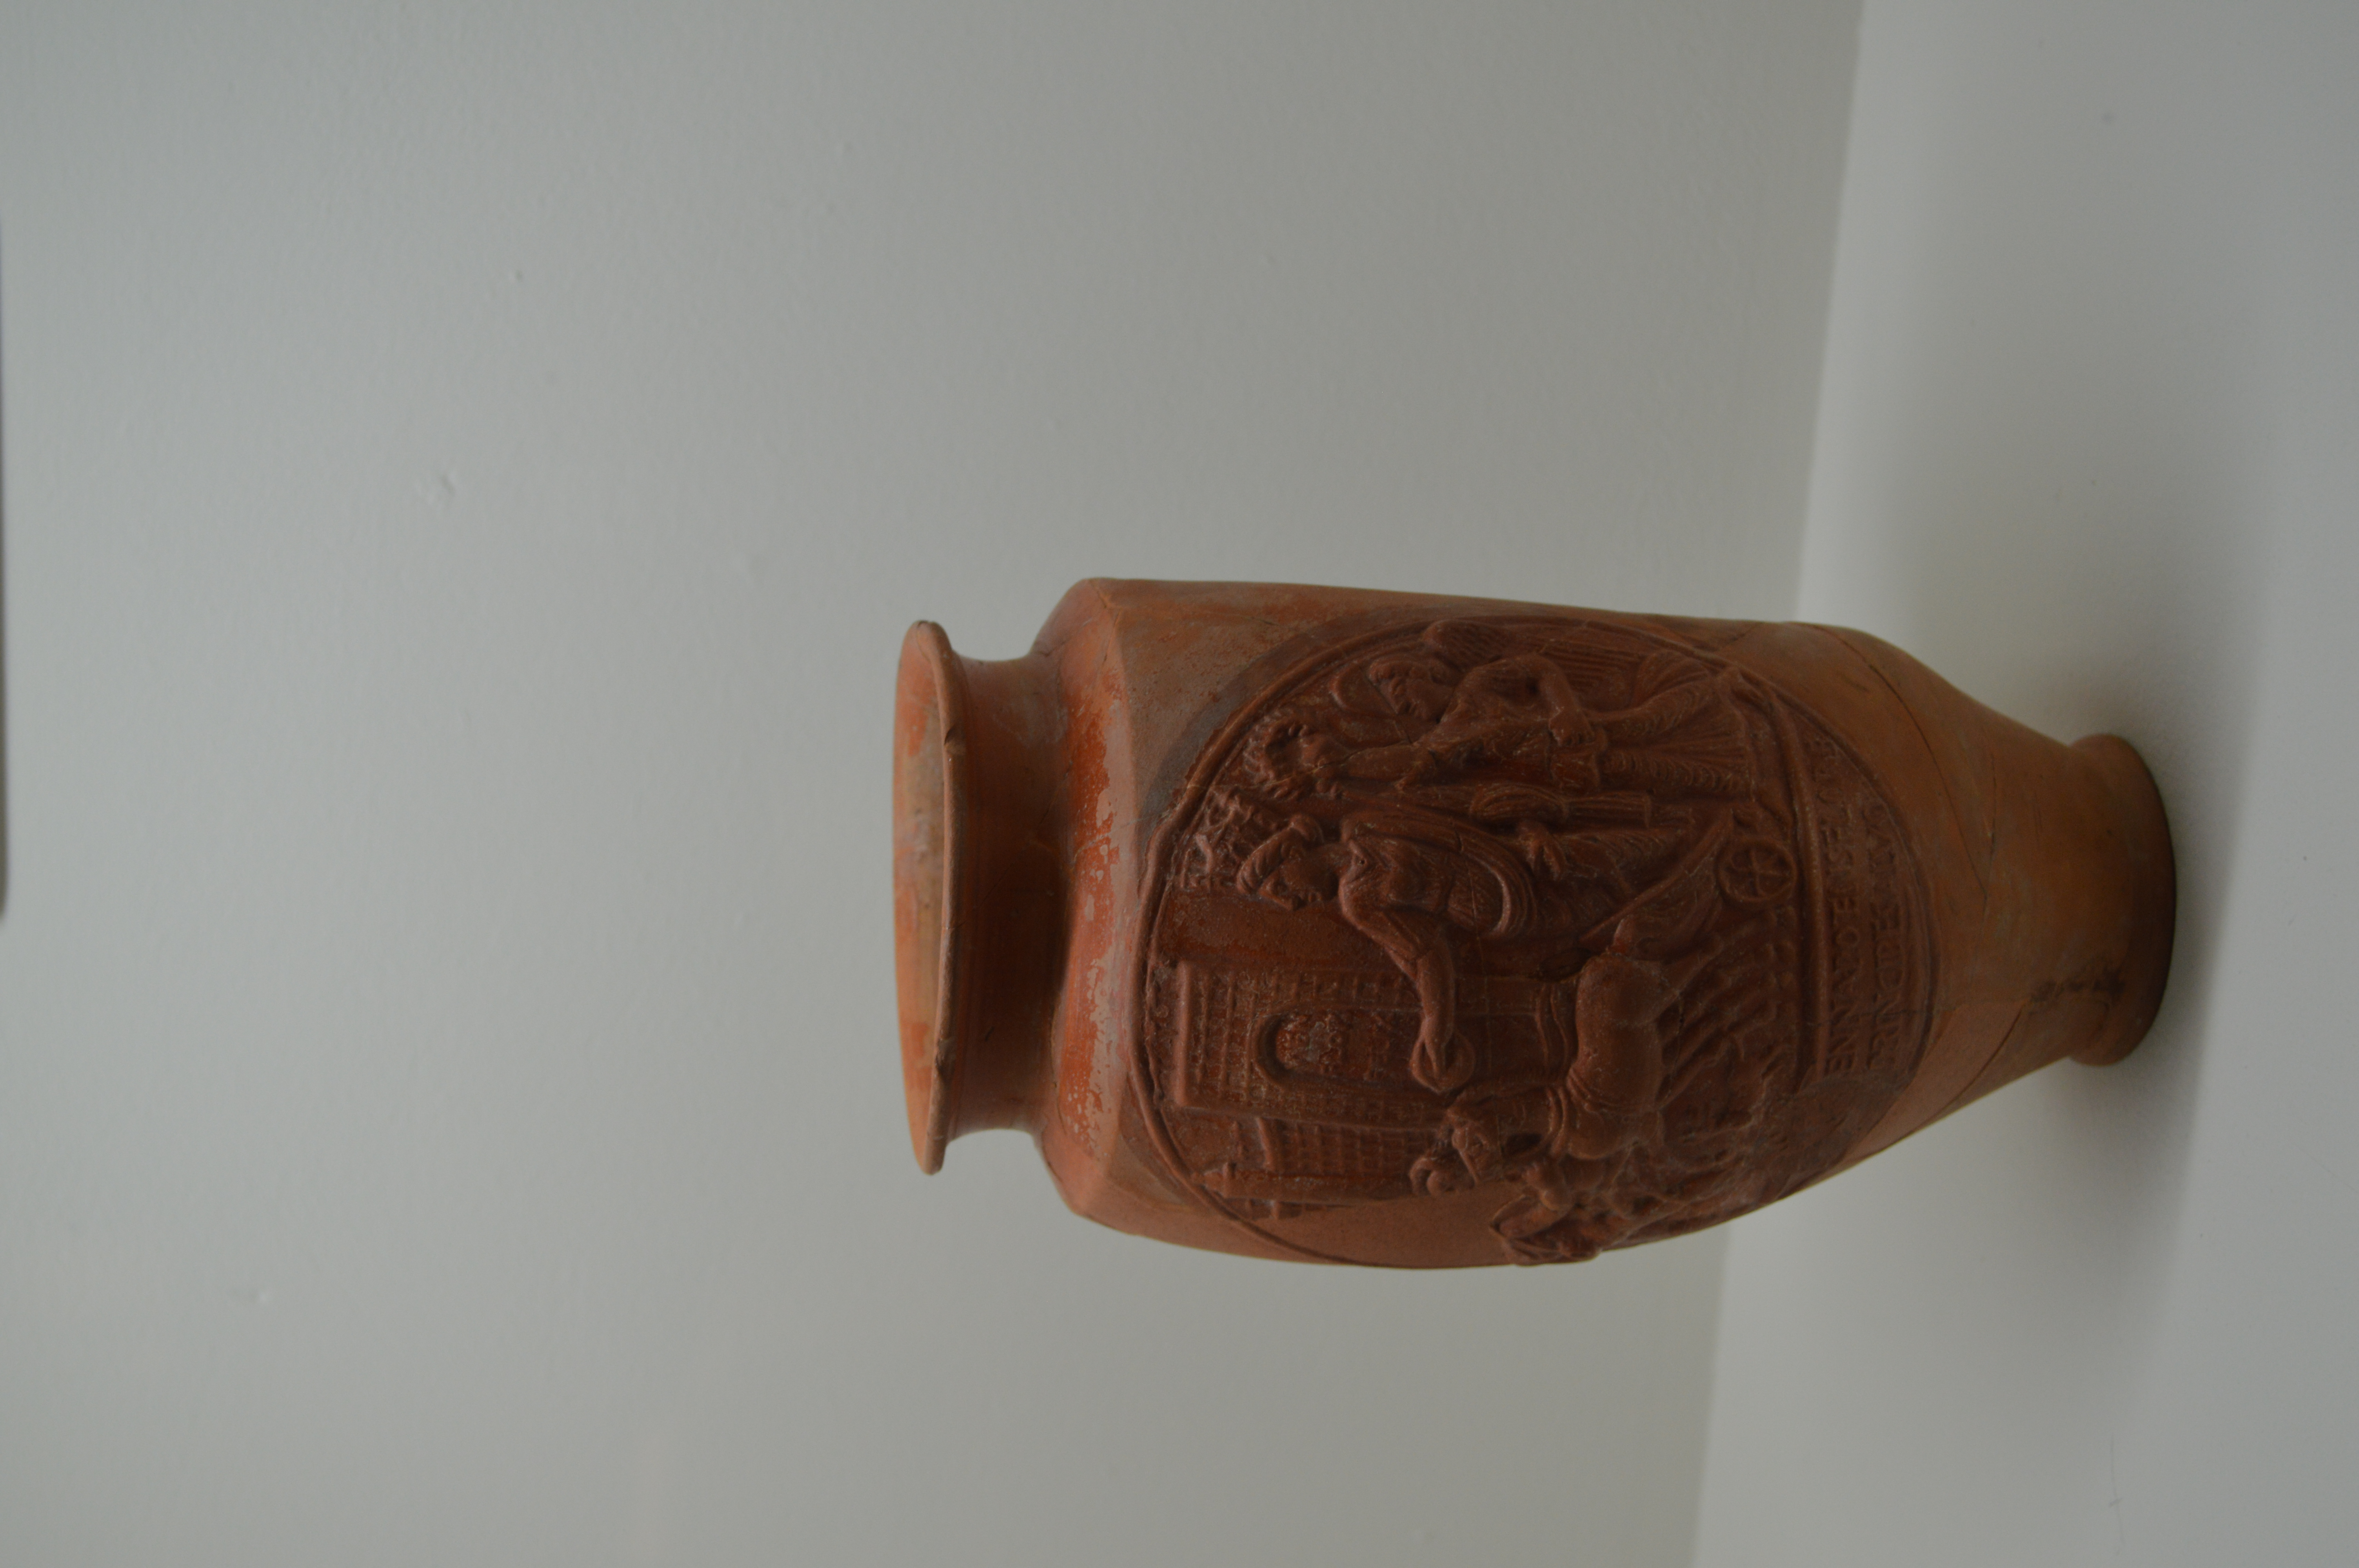
\includegraphics[height=\linewidth,angle=-90]{figures/DSC_0174.JPG}
   \end{minipage}
    \caption{Photographies de la collection de Fourvière. De gauche à droite: une stèle, une statue et une poterie.}
  	\label{fig:exempleFourviere}
\end{figure}

La collection appelée {\bf GaRoFou}, pour musée {\bf Ga}llo {\bf Ro}main de {\bf Fou}rvière, est composée d'images fixes (GaRoFou\_I) et de vidéos (GaRoFou\_V).

\subsubsection{Garofou\_I}
\label{subsubsec:garoufoui}

GaRoFou\_I contient au total 1252 photographies, prises par des appareils reflex, de 311 œuvres. Parmi ces images, 1068 sont des images du corpus, et 184 des images requêtes sélectionnées aléatoirement. Sur les 311 œuvres, 166 sont représentées dans l'ensemble des requêtes. Les photographies requêtes ont différents points de vue, qui ne sont pas forcément présents dans le corpus. Chaque image du corpus est identifiée par l'œuvre qui y est visible, auquel est associé le {\it type} de l'œuvre parmi: stèle (roches gravées, colonnes, ...), statue (sculptures, reliefs, ...), poterie, et autres (pièces, joaillerie, ...). Les œuvres sont identifiées par un triplet numéro de niveau (de A à D), le numéro d'œuvre dans le niveau, et un numéro d'image de l'œuvre suivant le format suivant:$<$numéro de niveau$>$$\_$$<$numéro de l'œuvre$>$$\_$$<$numéro d'image de l'œuvre$>$. Les images d'une même œuvre sont donc identifiées spécifiquement. 

\subsubsection{Garofou\_V}
\label{subsubsec:garoufouv}

La partie vidéo de la collection Garofou est composée de 11 vidéos qui correspondent à des visites de différents étages du musée. Ces visites ont été effectuées par 5 personnes différentes, le même jour, avec une caméra fixée au dessus de la tête. Le détail sur ces vidéos est présenté dans le tableau~\ref{tab:video_garofou}. Dans ce tableau, nous détaillons en particulier les étages (notés de $A$ à $D$) du musée, la durée totale des vidéos brutes dans lesquelles les personnes ne sont pas forcément devant une œuvre, les durées durant lesquelles l'annotation manuelle a déterminé que des œuvres étaient le centre d'intérêt des visiteurs, le nombre d'œuvres correspondantes qui peut contenir des redondances car une personne peut se focaliser plusieurs fois sur une œuvre, ainsi que le nombre d'œuvres uniques vues.
Associé à chaque vidéo, les objets visibles qui ont attiré l'attention du visiteur sont indiqués par leur horodatage d'apparition et de disparition (en {hh:mm:ss} par rapport au début de vidéo). Pour générer ces annotations, nous avons développé une interface spécifique sur la base de la structure d'annotation du projet CAMOMILE~\cite{poignant2016lrec}, dont un exemple est présenté en figure~\ref{fig:annotation}.

\begin{table}[htb]
    \centering
    \begin{tabular}{| c | c | c | c | c | c |}
    \hline 
    étage & \# vidéos & durée  & durée avec & \# d'œuvres & \# œuvres  \\
      	  &           & totale & œuvre      & regardées   & uniques 	   \\
    \hline    
    \hline    
    A & 4 & 66'55''  & 38'35'' & 157 & 59\\
    B & 2 & 31'21''  & * 14'44'' & 77 & 56\\
    C & 3 & 30'51''  & * 17'35'' & 63 & 37\\
    D & 5 & 57'34''  & * 25'06'' & 115 & 63\\
    \hline    
    \hline    
  	total & 11 & 186'41'' & 96'00'' & 412 & 215 \\
    \hline
    \end{tabular}
    \caption{Vidéos de la collection GaRoFou\_V.}
    \label{tab:video_garofou}
\end{table}

\begin{figure}
\centering
    \includegraphics[width=0.9\linewidth]{figures/annotation.png}
    \caption{Interface d'annotation des vidéos. En haut: l'affichage de la vidéo, en bas chaque segment annoté de vidéo avec l'identifiant d'objet.}
   \label{fig:annotation}
\end{figure}

De la partie annotée de cette collection sont tirées des images fixes : chaque segment (suite d'images contiguës temporellement) annoté a été découpé en, au plus, 10 sous-segments de 1 seconde répartis régulièrement et sans chevauchement. De chaque sous-segment, l'image la plus nette est sélectionnée par recherche plus grande variance de couleurs après application d'un opérateur laplacien. Pour évaluer les systèmes, chacune de ces images extraites d'un visiteur est utilisée comme requête face aux images extraites issues des visites des autres visiteurs (validation croisée par visiteur). Nous conservons dans les requêtes uniquement les œuvres qui ont été vues par au moins deux visiteurs. 
Le tableau~\ref{tab:video_garofou_visiteur} récapitule les données quantitatives liées aux images extraites de GaRoFou\_V, par utilisateur : nous détaillons en particulier le nombre de segments utilisés pour extraire les images annotées qui servent à réaliser les évaluations.

\begin{table}[htb]
    \centering
    \begin{tabular}{| c | c | c | c | c | c | c | c | }
    \hline 
    visiteur & \# vidéos & durée   & durée avec &\# segments   & \# d'œuvres & \# Images & \# Images \\
      	     &           & totale  & œuvre      & annotés    & uniques     & total     & requêtes  \\
    \hline    
    \hline    
    u1       & 2         & 48'54'' & 22'22''    & 115        & 101        & 768       & 625       \\
    u2       & 1         & 24'25'' & 14'8''     & 62         & 51         & 493       & 444       \\ 
    u3       & 4         & 63'44'' & 24'36''    & 153        & 141        & 964       & 624       \\ 
    u4       & 1         & 10'50'' & 2'24''     & 13         & 11         & 101       & 101       \\ 
    u5       & 3         & 38'49'' & 16'1''     & 69         & 60         & 453       & 338       \\
    \hline
    total    & 11        & 186'41''& 79'30''    & 412'       & 215        & 2779      & 2132      \\
    \hline
    \end{tabular}
    \caption{Images requêtes issues des vidéos du corpus GaRoFou}
    \label{tab:video_garofou_visiteur}
\end{table}

\subsection{Récapitulatif}
\label{subsec:recap}

Nous remettons en perspective dans le tableau~\ref{tab:recap_corpus} les deux collections que nous avons construites, en fonction des critères définis en section~\ref{sec:desc_corpus}. 
Nous remarquons en particulier que nos collections sont intéressantes du point de vue de la quantité d'instances à retrouver, et aussi sur la variation des images de requêtes (images fixes ou vidéos).

\begin{table}[htb]
    \centering
    \begin{tabular}{| c || c | c | c |}
    \hline 
    & Clicide & \multicolumn{2}{|c|}{Garofou} \\
    \hline
    &  & Garofou\_I & GaRoFou\_V \\
    \hline 
    \hline
    objet & Peintures (2D) & 2D et 3D &  2D et 3D \\
    \hline    
    média & Images fixes & Images fixes  & vidéos \\
    \hline
    acquisition & contrôlée &  contrôlée  &  contrôlée \\
    \hline
    taille (C/Q) & 2500 / 512 & 1100 / 172 & 2779/2132 \\
    \hline
    \end{tabular}
    \caption{Caractéristiques des collections proposées}
    \label{tab:recap_corpus}
\end{table}

Afin d'estimer l'utilité de ces deux collections pour la communauté de recherche d'images et de vidéos, nous allons étudier en partie~\ref{sec:eval_reco} la qualité des résultats obtenus par des approches emblématiques de l'état de l'art.



\chapter{Corpus d'images et de vidéo pour la recherche d'instance}

\section{Création d'un corpus d'image pour la recherche d'instance}

\section{Création d'un corpus de vidéo pour la recherche d'instance}

\section{Annotation et Indexation}

